\chapter{Introduction}

%% INTRO
Despite that modern \textsc{Graph Database Management Systems} (GDBMSs) are a well-known subject of studies, three fundamental aspects are missing in literature: operators integrating and combining graphs, the adoption of such operators in current graph query languages, and the definition of a graph data structure providing both a multidimensional and nested representation. As regards of the aforementioned graph integration operators, both graph joins generalizing the graph products and graph nestings summarizing graph data with other extracted graph patterns are required. 


% current literature and already-existing systems do not allow to integrate graph data with other semistructured, structured or unstructured data . In particular, a query language allowing the transformation and cleaning of such different sorts of data is missing. 



\begin{figure}[!p]
	\begin{minipage}[b]{\textwidth}
	\centering
	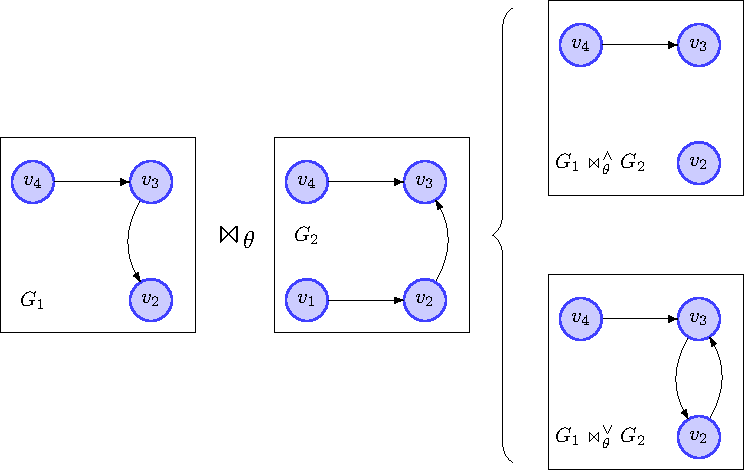
\includegraphics[scale=0.7]{fig/00introduction/g1g2_general_conjdisj}
	\subcaption{This picture provides two different possible evaluation of the graph join operator: in both cases, given the graphs operators $G_1$ and $G_2$, the matched vertices are merged together into one single vertex. Over this basis of matching vertices, the way to combine the edges between these matched vertices may vary. In particular, we will later on present the conjunctive ($\wedge$) and the disjunctive ($\vee$) ``semantics'' for combining such edges.}
	\label{fig:introducingJoins}
	\end{minipage}
	\begin{minipage}[b]{\textwidth}
	\centering
	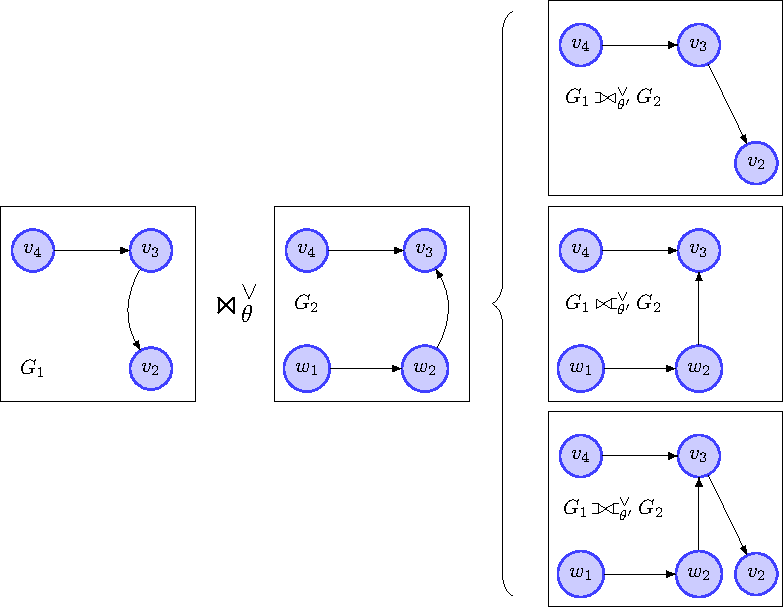
\includegraphics[scale=0.7]{fig/00introduction/g1g2_general_disjleftright}
	\subcaption{Given two graph $G_1$ and $G_2$, we provide the result of 
		three possible outer joins over the disjunctive graph join: vertices sharing the same id identify
		vertices with a same value. 
		These figure make explicit that the left/right full outer interpretation returns both the vertices that
		are shared among the graphs and the vertices belonging to the left/right graph.}
	\label{fig:conjdisjbasicexouter}
	\end{minipage}
\caption{Introducing Graph Joins over standard graphs.}
\end{figure}
%In order to provide such general framework for data integration, 

In particular, this thesis is going to focus on two graph operators allowing to combine graphs: \textbf{graph joins} and \textbf{graph nestings}. First, the graph join operator (Chapter \vref{cha:join}) is useful in practical scenarios, such as the intersection or the merge of different transport overlay networks, or for comparing and merging different ontology representations. The flexibility of such operator at the edge combination level permits such scenarios (Figure \ref{fig:introducingJoins}). Moreover, if we fix a same theta-join predicate and a specific edge semantics, we could further on extend the definition of the graph join as in the relational model, that is by allowing that even the non matching vertices from one (left and right join) or both operands (full join) must also appear (Figure \ref{fig:conjdisjbasicexouter}). Hereby, the graph join operator defines a whole class of graph operators (\textbf{graph $\otimes_\theta$-products}), that can be differently instantiated as required by the user, and hence can be also differently implemented. 

Graph nesting (Chapter \vref{cha:nesting}) permits the summarization of graph data within one graph data source: in particular, we could ``fuse'' or ``summarize'' all the vertices belonging to the same cluster, and then we could group the paths occurring between the fused vertices as edges containing such paths. As a consequence, such operator provides dimensionality reduction that is often required in multidimensional data analysis. \textsc{Group Recommendation Systems} characterize a use case scenario  in which the members sharing similar interests and their suggested activities could be ``fused'', thus providing a coarser representation of the sequence of similar activities.  While the class of graph join operators can be defined on top of current graph representations, graph nesting requires an extension of the graph data model for fulfilling the aforementioned graph data integration purposes. Such extension must allow to represent graphs within both vertices and edges (nestings), thus representing a summarized view of the contained graph. Nested representations are shared among task representations and complex world knowledge representations, such as medical procedures for specific diseases such as glaucoma \cite{NestedGlaucoma}. 
\bigskip

Graphs distinguish two different classes of data types, vertices and edges. Edges are constrained by the ids of the vertices through source and destination dependencies. In particular, most graph operators require the execution of distinct operations over the vertex and edge sets. Nevertheless, current graph data structures do not allow a direct data integration with semistructured data  \cite{Pentaho,Parra} (and hence, even structured data) because graph definitions such as property graphs and RDFs do not permit nested representations, neither in vertices  nor in edges. Hence, direct data manipulation allowing to directly integrate graph data with semistructured data are not possible.  %Although some Data Warehouses provide multidimensional characterization of structured data, and some DBMSs support multiple data representations (graph based, structured, semistructured and genetic data: \textit{Oracle Database} \cite{Loney08} and \textit{OrientDB} \cite{OrientDBMed}) that are homogeneously queryable using a same conventional query language, such solutions still do not provide a solution for integrating data which is either schemaless or has different kind of schema.
\textit{Expert systems} are an example of practical use cases requiring the features in the previous generalized data integrations; such systems could be either general purpose (such as \textit{IBM Watson} \cite{IBMWatson} and \textit{DeepDive} \cite{PalomaresAKR16}) or more domain knowledge related, such as healthcare settings (medical diagnosis formulation \cite{NestedGlaucoma} and health condition prediction methods \cite{OPLON15}). 
For this reason the present thesis proposes a new graph data model, named \textbf{nested graphs}\index{nested graph}, allowing the embedding (or \textit{nesting}) of both vertices and edges for both data class types, hence permitting graph nesting operations. Nested graphs allow to directly represent semistructured documents. In particular, such data model  relies on a broader semistructured model, \textsc{General Semistructured Model} (\textbf{GSM}), which both overcomes current  data models' limitations and is proposed by this thesis. 



Last, we must ask ourselves which is a proper language to query nested data structures, including nested graphs: given the aforementioned considerations, such query language should be able to  express queries for both (semi)structured and graph data. In order to complete the data integration of (semi)structured with graph data, such language should  express  data transformations  towards the most general data representation - our nested graphs - and to uniform the sources' data schema in one single user-provided final schema. In order to meet such research goals, this thesis proposes the \textbf{GSQL} query language over GSMs, thus allowing to formally characterize the \textsc{Global as A View} data integration scenario in its entirety. The graph join and nesting operator, the definition of a graph query language for data integration and the outline of a data integration system for any sort of data representation are all required features missing in current literature, which are provided by the current thesis. In particular, the adoption of these solutions allows to achieve these further outcomes:
\begin{itemize}
	\item A new property graph representation allowing to optimize the graph join operators by exploiting primary and secondary indices. This data structure also allows an easy parallelization by splitting the data in different vectors. This data structure is extended to efficiently support a nested data representation.
	\item Current  query languages optimization strategies do not  efficiently implement  graph joins and nestings. The definition of graph joins in current query languages is  verbose, while the proposed graph join definition provides a more user-friendly representation.
	%\item \hl{The graph nesting operator should be implemented in a distributed environment}. 
	\item The definition of GSQL (Chapter \vref{cha:NGQL}) allows the expression within the same syntax of both graph and semistructured pattern query languages, alongside with set, relational and semistructured operations. On the other hand current graph query languages often provides these features singularly at an higher abstraction level.
	\item GSQL query language allows the implementation of all the data integration operators required in the \textsc{Global As A View} approach.
\end{itemize}


\section{Graph Data: Use Cases}
Graph databases are already used in tasks requiring the  integration of both schemaless (or time-variant schema) data alongside  with structured information  \cite{Petermann2014,SoussiAZ11}. Graphs are used as an intermediate
representation during the data transformation phase, thus allowing to
integrate intermediate graph representation with other graph data.
In addition to Social Networks \cite{DMR}, graph data is also used in the following scenarios:

\begin{description}
	\item[Analysing (Hyper)texts.]
	Even if hypertext contents are usually provided as semi-structured data using markup languages like XML,
	some recent work  proposed alternative graph representations. 
	\medskip
	
	Firstly, if
	we want to focus on the mere syntactic representation of  semi-structured data, we could analyse how the
	author used the XML tags to produce the document, and investigate which structural patterns were used.
	In this case an RDF representation 
	\cite{Lassila1999,GutierrezInclusion}
	provides a ideal schema-independent data  \cite{IorioHierarchy,BarabucciEARMARK} that could be used in automatic reasoners such as \textbf{Jena} \cite{Jena} and \textbf{Pellet} \cite{Pellet} to extract
	structural informations.
	\medskip
	
	Finally, graphs can provide a semantic interpretation of the textual content
	 \cite{Iglesias}. Such representation allows to later
	perform either specific graph mining algorithms \cite{Samatova} such as clustering and association rules,
	or basic graph metric operations such as betweenness centrality and degree distribution \cite{Newman}.
	In this context, graphs are also used  to represent  knowledge bases
	such as \textbf{BabelNet} or \textbf{WordNet}, for
	multi-word recognition \cite{Lossio-Ventura2014}, word similarity \cite{SemSim} and multilingual
	word disambiguation \cite{MultiWordSense}.
	
	\item[Temporal Data.] One of the problems\footnote{See Section \vref{sec:relreprprob} for further problems related to the relational model.} of the relational model is its inability to represent temporal data. Many possible representations for temporal graphs structures have been proposed.
	The most simple data model is to represent the evolution of a network through time via distinct graph
	snapshots \cite{AnIntroductionGraph}. This multi-layer network model is
	not very informative since no information is provided to understand how the different layers are related to
	each other.
	
	Temporal information can be represented as a single graph \cite{Wu}: 
	each vertex represents an agent and each edge expresses an interaction, which time span is represented through the edge's weight. Such representation suffers from interpretation problems: firstly, when cyclic
	interactions occur it is not clear which node started the communication process, and secondly,
	 nodes  having different interaction times are not taken into account.
	
	All those issues are
	solved by another multi-layer graph representation \cite{Kostakos2008}, where each layer describes the snapshot
	of the interactions occurring at a given time, while the extra-layer edges link the same agents interacting
	subsequent time steps.
	
\item[MOLAP representation.] \label{molap} %Graph databases are already used in 
Business Intelligence applications may also use %for integrating either schemaless data or data which schema varies
%in time and still, their integration with structured information is required. 
graph databases for  % are used as
MOLAP multi-dimensional  data warehouses, in which different types of data are %where such kind of data is 
integrated \cite{Petermann2014,SoussiAZ11}. Given that vertices can be associated to distinct dimensions \cite{PterMicBergami}, graphs allow
data warehouse multidimensional queries  \cite{ChenYZHY08,Zhao11,Etcheverry2012a}. Companies are already
generating graph data as Enterprise Social Networks, which are used as an infrastructure for internal communication and
opinion mining. Graphs allow the measurement of enterprise
success \cite{success} and to design company workflows \cite{Park2016355}. 
Such enterprise graph data could be integrated with  external business-oriented OnLine Social Networks (e.g. LinkedIn, Ask-a-peer).

\end{description}
